\section[History of Modular Synthesizers]{History of Modular Synthesizers}\label{section:mod-synth-history}

\begin{figure}
  \centering
  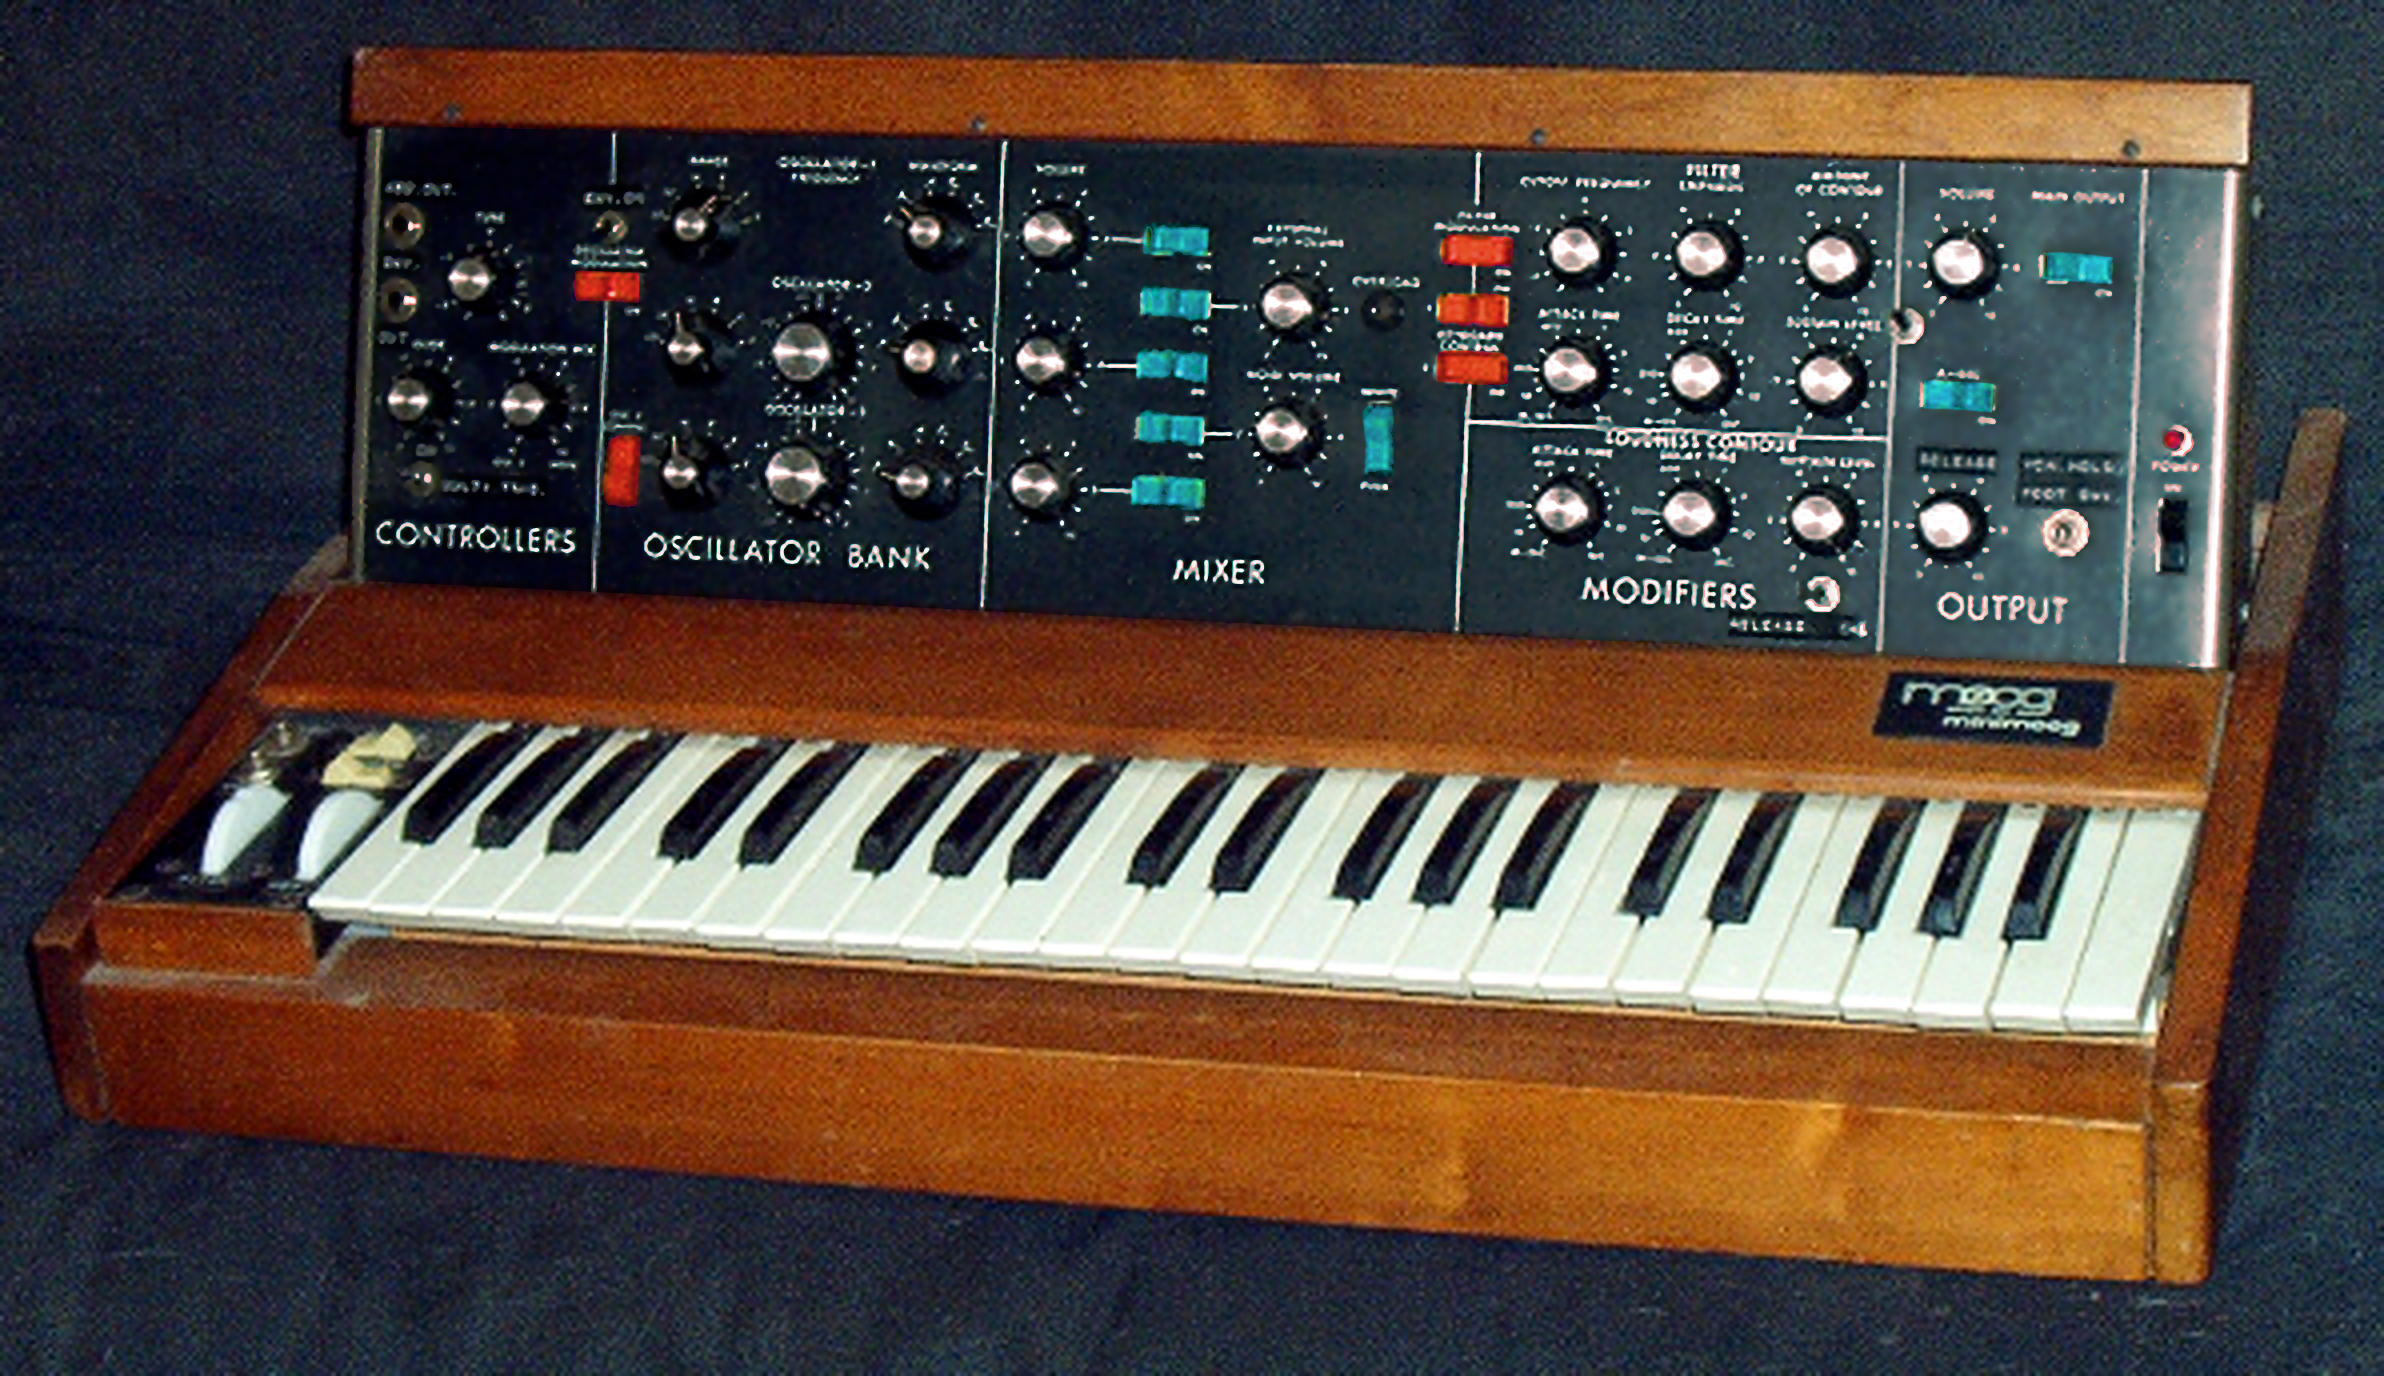
\includegraphics[width=\textwidth]{Minimoog.jpeg}
  \caption{The Minimoog Model D}
  \label{fig:minimoog}
\end{figure}

\begin{figure}
  \centering
  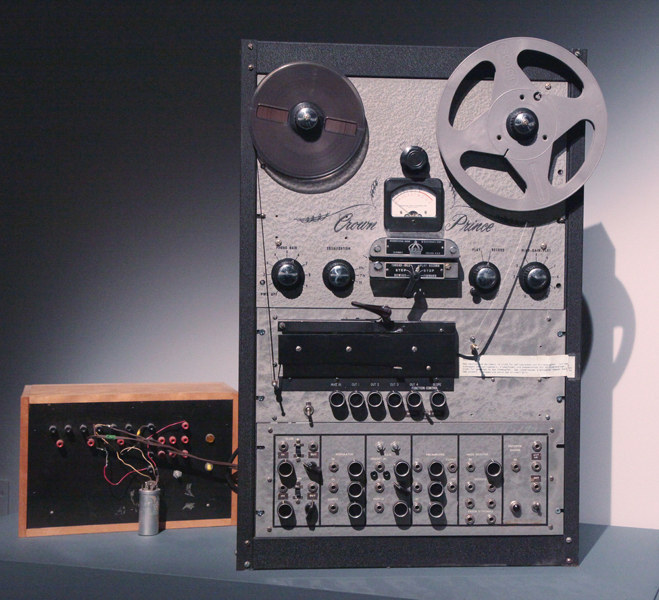
\includegraphics[width=0.5\textwidth]{bode-audio-system-synthesizer.jpeg}
  \caption{The Bode Audio System Synthesizer}
  \label{fig:bode-audio-system-synthesizer}
\end{figure}


The 1950s was a turning point within the field of electronic music and communicational technologies. This marked the creation of electronic music, with the use of physical components. Electronic music was rare, with synthesizers and electronic instruments (examples of which include the electric guitar, electric keyboard, electric bass guitar, and more) being less common. Modular synthesizers were also rare, at that point they contained fewer modules than found in modular synthesizers today. These modular synthesizers were large, taking up significant space, as evidenced by Bode's Audio System Synthesizer (Figure \ref{fig:bode-audio-system-synthesizer}) \cite{Crab_2019a} \cite{Says_2014} and Moog's Minimoog Model D (Figure \ref{fig:minimoog} \cite{Krash_2005}) \cite{Pinch_Trocco_1998} \cite{Pinch_Trocco_2004}, two influential analog modular synthesizers.

The first module, or functionality, created was the positive feedback oscillator, sometime between 1912 and 1914 \cite{Gabrielli_2020}, a module now commonly found in modular synthesizers, both in analog (physical) and digital (virtual) synthesizers. A positive feedback oscillator--or as it is known today, the oscillator--produces sound in which the output varies up and down (it oscillates) in a repeating pattern \cite{Meyer_2016}.  This is where the oscillator module gets its name, producing a sound which rises and falls, or oscillates. The resulting sound an oscillator produces will typically be one of four fundamental waveforms: the sine wave, triangle wave, sawtooth wave, square wave, or less commonly, the pulse wave. The creation of this positive feedback module is attributed to Austrian engineer and physicist Alexander Meissner. Unlike the oscillator module found today, the early version was only able to last a few minutes. Instead of continuously able to produce an audio waveform, this version produced only a small output of power \cite{Fleming_1919}. 1912 introduced the communicational technologies field as something more than niche. Products from proper physics laboratories were rare to find, and so were machines capable of producing audio waveforms with high frequencies after several minutes. Meissner created a new type of machine: a high-frequency generator from an amplifier, with a vacuum tube as a substitute for a high-frequency receiver machine \cite{Fleming_1919}. Previous to Meissner's creation, it was impossible to establish a connection between a high-frequency machine with a receiver. The output frequency of such a machine was not the same as the user's desired output frequency, a synchronous and superimposed frequency. Meissner's product was easier to handle than these machines, and much more useful. In addition, Meissner's machine was much less noisy as well. This machine could change the output frequency given to the receiver, and tune the receiver machine to a range of wavelengths that were previously not possible \cite{Fleming_1919}. This development changed the process of receiving wavelengths, and resulted in the un-dampened wave. An un-dampened audio wave is the typical audio wave which oscillates without any force or opposing motion to prevent it from oscillating. This differs from a dampened wave, which is an audio wave which oscillates, yet there is some force or opposing motion which slows the wave, or stops it completely. Eventually, the dampened wave will lose energy, such that it will stop oscillating, unless there is an external force or motion to cause the wave to continue to oscillate. This un-dampened audio wave which resulted allowed for a user to fine-tune the frequency, while also suppressing any atmospheric distractions or sounds. With Meissner's work, the field's knowledge of constant sound generation and high frequencies was expanded, and paved the way for future work on the short-wave band \footnote{Though not discussed in this paper, the short-wave band is typically used in maritime communications, international, and radio broadcasting. More reading on Alexander Meissner and his patented solution can be found in the Engineer and Technology History Wiki's page on Alexander Meissner here: \url{https://ethw.org/Alexander_Meissner}}.

\begin{figure}
  \centering
  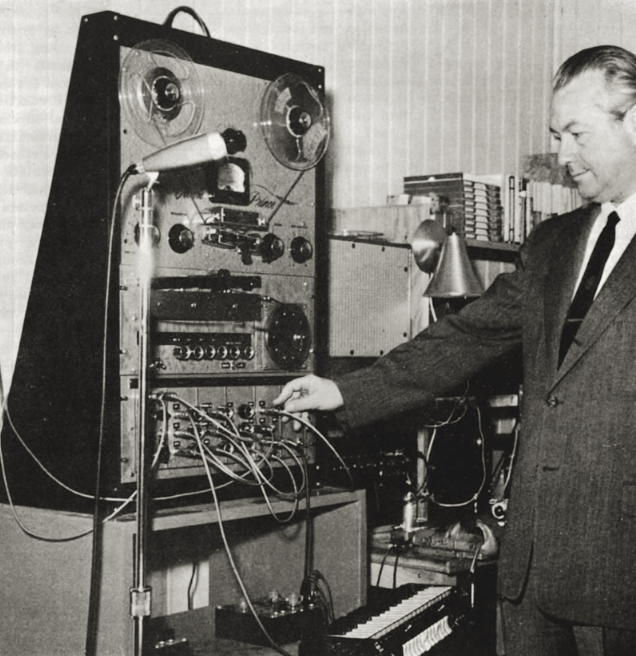
\includegraphics[width=0.5\textwidth]{harold-bode.png}
  \caption{Harold Bode demonstrating the Bode Audio System Synthesizer}
  \label{fig:harold-bode}
\end{figure}


Then, sometime between 1959 and 1960, Harold Bode (1909-1987), a German engineer, created the modular synthesizer which we are familiar with today. Bode was a German engineer and designer of audio tools. He foresaw that transistor technology (a semiconductor device which is used to amplify, control, and generate electrical signals) would become a key change in creating and designing synthesizers, especially modular synthesizers\cite{Gabrielli_2020}. Transistors would link the audio signal through cables, through where each component, or \say{module} could be connected in any order, according to the user's preferences. Multiple modules--including modulators, filters, reverberation generators, and more--could then be connected in any order, either to modify or generate sounds. With transistor technology, Bode created his \textit{Audio System Synthesizer} (Figure \ref{fig:harold-bode} \cite{Crab_2019b}), which allowed for a larger number of sound creation possibilities than before. The system itself contained inputs for various sound sources, and the input signals could be modified by filter modules and a modulator\cite{Bode_1984}. As the system was modular, there were independently working modules for sound modification. These modules could be combined with each other in several ways, according to the user's desired order. This Audio System Synthesizer also made an impression on Robert Moog, who would take Bode's idea and further develop it \cite{Gabrielli_2020}. 

Robert Moog (1934-2005) was an American engineer inspired by Harold Bode's Audio System Synthesizer. As the inventor of the first commercial synthesizer, dubbed the Moog synthesizer, Moog created the first integrated synthesizer (a synthesizer in which the modules are integrated into the system itself, rather than needing to be connected through cables). The Moog synthesizer was built in 1964, and contained several of the fundamental synthesizer concepts found today\cite{Pinch_Trocco_2004}. These modules on the Moog synthesizer included the voltage-controlled oscillator, voltage-controlled filter (a module which reduces or outright removes certain frequencies and harmonics from sound that is passed through \cite{Meyer_2016}), envelope generators (a module which is used to shape the volume, or dynamics of a note when connected to an amplifier module, as well as alter the frequency or timbre of a note if connected to a filter module \cite{Meyer_2016}), and the pitch wheel. With the Moog synthesizer, synthesizers were brought to a wider audience, influencing the development of popular music\cite{Pinch_Trocco_2004}. What followed the Moog synthesizer was the Minimoog Model D (Figure \ref{fig:minimoog} \cite{Krash_2005}), a portable 1970 creation. The Minimoog Model D is acknowledged to be the most \say{influence synthesizer of all time}\cite{Gabrielli_2020} due to its playability and compactness. Similar to the Moog synthesizer, it included modules to both generate and alter sounds \cite{Pinch_Trocco_2002}.

The 1960s also saw the introduction of Donald \say{Don} Buchla, and his Buchla 100 Series Modular Electric Music System. Don Buchla (1937-2016) was another American inventor, working in the field of sound synthesis independently of Robert Moog. The Buchla 100 Series (otherwise known as the \say{Buchla Series 100} or \say{Buchla Box}), is a keyboard-less modular synthesizer. Unlike Moog's Moog synthesizer and Minimoog Model D, the Buchla 100 Series used a more manual control\cite{Pinch_Trocco_1998}. Instead of a keyboard for user input, the user would control the synthesizer's modules directly. It contained a logical layout, with an intuitive, user-facing front panel, which allows the user to directly patch and route modules together, using patch cords. With the various knobs and triggers on the synthesizer itself, a user could manipulate sound according to multiple parameters. Along with user input differences, there were other important distinctions between the Buchla and Moog synthesizers. These changes include Buchla's use of voltage-controlled oscillators with multiple complex modulation options, and a decrease in emphasis on using filters. This methodology would lead to a division in school of thought: the East Coast school of thought, and the West Coast school of thought \cite{Gabrielli_2020}. The West Coast method, which was led by Buchla, put greater emphasis on the experimental side of electronic music, and so designed their synthesizers according to this.

Both the East Coast and West Coast methods of audio synthesis are important, as they eventually become the two general methods for synthesis: additive synthesis and subtractive synthesis (two other types of audio synthesis, to be explained in section \ref{section:modular-synth-what-is}). In a general overview, the East Coast approach embodies a straightforward and practical approach, with efficiency and reliability as important concepts, while West Coast synthesis focuses on experimentation and the inclusion of non-tradition modular controllers such as the touchpad \cite{Meyer_2016}. For East Coast audio synthesis, its patches and way of forming modules fall under the category of \say{subtractive synthesis}. Subtractive synthesis involves starting with a complex audio waveform, with multiple harmonics (i.e. pitches, or notes)\cite{Winer_2018}. Then, a low-pass filter (or in analog synthesizers, a voltage-controlled low-pass filter, or VCF) slowly removes selected frequencies from the complex wave. The sound produced by West Coast synthesis is less known that East Coast synthesis. In place of aspiring towards a sense of musical efficiency, the West Coast method evolved out of the desire to replicate the acoustically-generated tones through manipulating previously recorded sounds\cite{Nielsen}. Thus, the West Coast method is not centered around a singular principle. It combines elements of additive synthesis (the addition of multiple, simple audio waveforms together to create a complex, composite waveform--often sine waves)\cite{Nielsen} and frequency modulation to create many sounds of complex timbres. Both additive and subtractive synthesis will be discussed further in the next section.
